% \begin{center}
%     \captionof{figure}{Bias in Contextual Effect for Different Estimation Approaches (with $N = 200, T = 5, \sigma_{X,\text{b}} = 3, \sigma_u = 0, \gamma_{01} = 3$)}
%     \begin{subfigure}[b]{\linewidth}
%         \centering
%         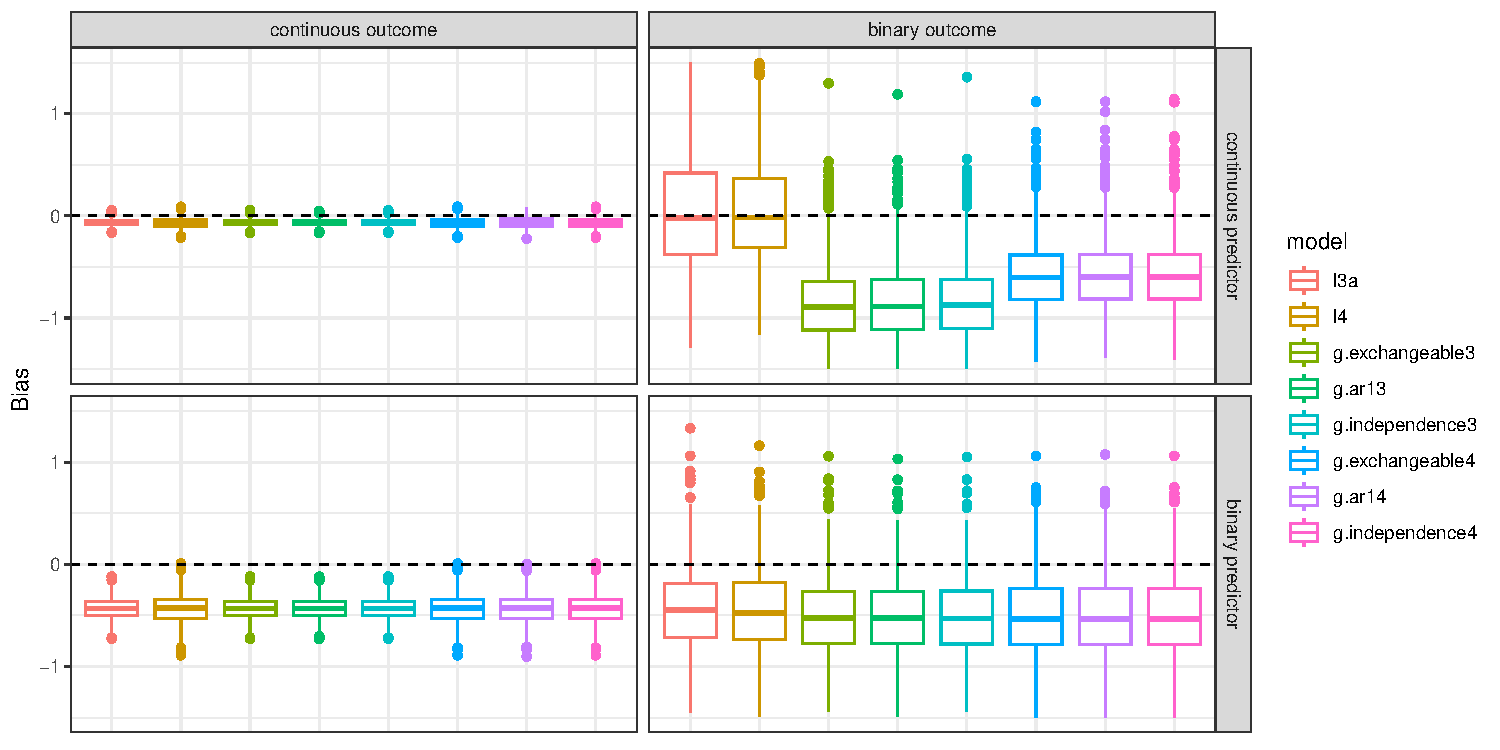
\includegraphics[width=\linewidth, keepaspectratio]{Figures/bias_plot_contextual_scenario1.pdf}
%         \caption{No Unobserved Heterogeneity ($\sigma_u = 0$)}\label{fig:results-contextual-scenario1}
%     \end{subfigure}
    
%     \begin{subfigure}[b]{\linewidth}
%         \centering
%         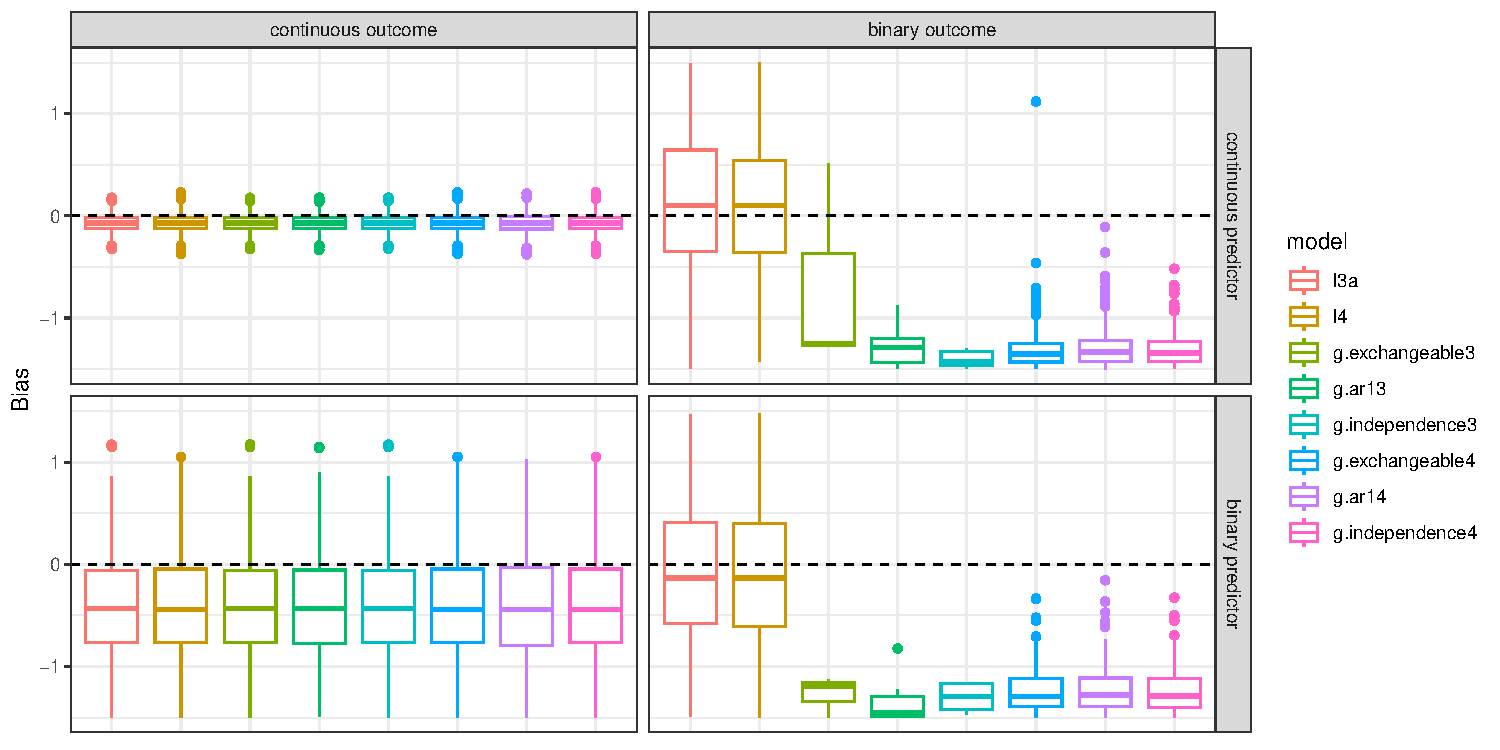
\includegraphics[width=\linewidth, keepaspectratio]{Figures/bias_plot_contextual_scenario2.pdf}
%         \caption{Large Unobserved Heterogeneity ($\sigma_u = 3$)}\label{fig:results-contextual-scenario2}
%     \end{subfigure}
%     \label{fig:results-contextual}
%     % \begin{figurenote}
%     %     \ldots
%     % \end{figurenote}
% \end{center}

% \newpage

\begin{center}
    \captionof{figure}{Bias in Contextual Effect $\gamma_{01}$ for Different Estimation Approaches for No and Large Unobserved Heterogeneity (with $N = 200, T = 5, \sigma_{X,\text{b}} = 3, \gamma_{01} = 3, \sigma_u = 0, 3$)}
    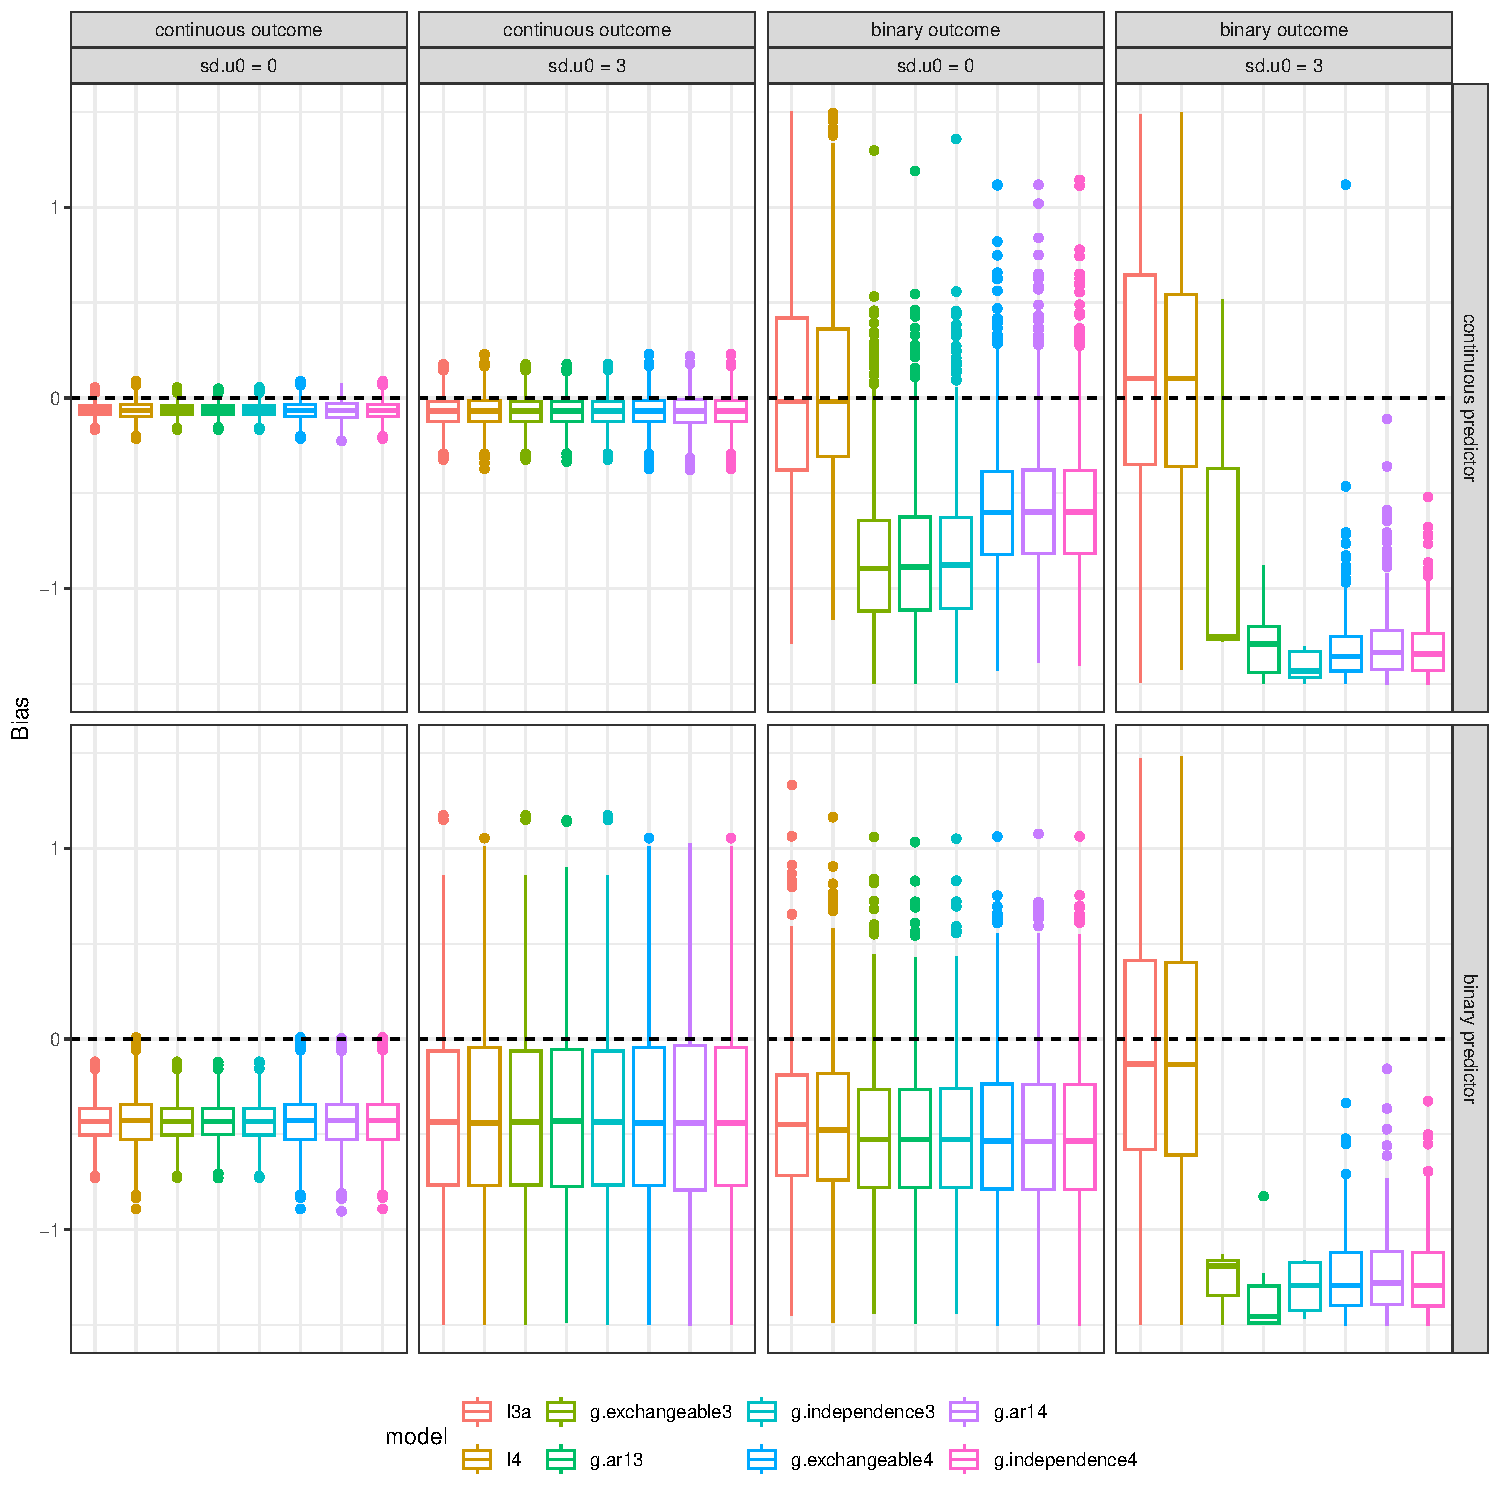
\includegraphics[width=\linewidth, keepaspectratio]{Figures/bias_plot_contextual_scenario3.pdf}
    \label{fig:results-contextual}
    % \begin{figurenote}
    %     \ldots
    % \end{figurenote}
\end{center}